\begin{figure}[!htbp]
  \centering
  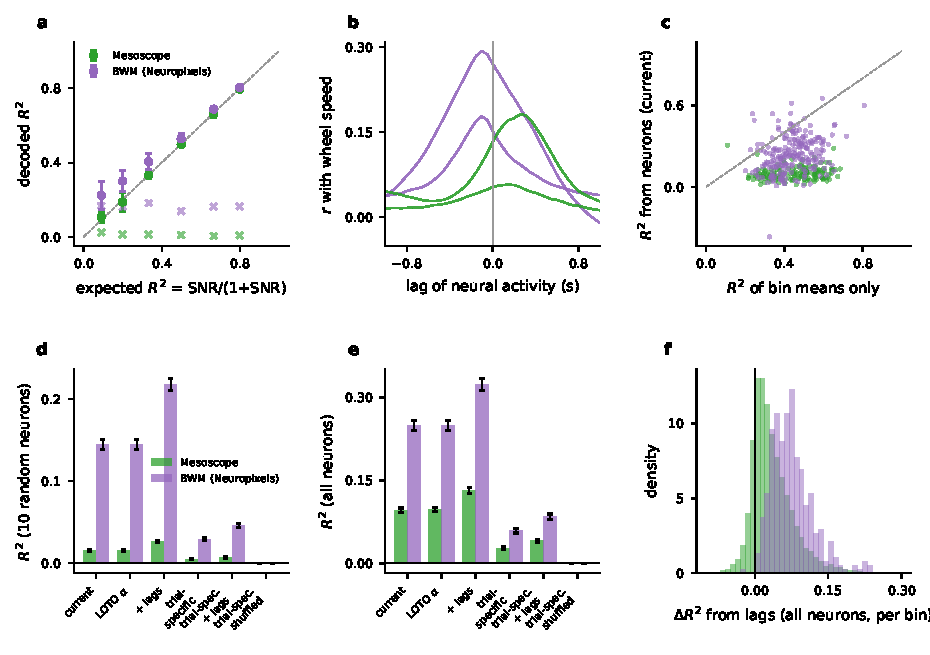
\includegraphics[width=\linewidth,height=0.8\textheight,keepaspectratio]{figures/checks.pdf}
  \caption{Checks of the wheel-speed decoding. The decoder and target are correct (after removing encoder glitches in 16 mesoscope sessions), mesoscope activity lags the wheel by about one 0.2\,s bin more than spikes, and the $R^2$ is dominated by the stereotyped speed profile after movement onset rather than by trial-to-trial differences in speed. \textbf{a} Decoder check: a synthetic neuron (wheel speed plus Gaussian noise at signal-to-noise ratios 0.1--4) replacing one of 10 random neurons of a session is recovered at the expected $R^2$ (dots: mean $\pm$ s.d. over 5 draws and 3 sessions per modality; crosses: the same 10 neurons without it). The decoder reproduces the dorsal-maps GPU decoder (max difference $2\times10^{-15}$) and the scikit-learn reference ($1\times10^{-7}$). The wheel-speed target agrees with brainbox's filtered speed ($r\geq$0.9999) once encoder glitches are removed. \textbf{b} Timing at full resolution: correlation of neural activity with wheel speed at lags $-1$ to 1\,s (positive: neural activity follows the wheel), mean over the 5\,\% most wheel-correlated neurons selected on the first half of each session and measured on the second half; 2 sessions per modality. Mesoscope deconvolved activity peaks 0.15--0.25\,s after wheel speed, BWM spikes 0.10\,s before it. \textbf{c} What the $R^2$ measures: predicting each bin from its mean over the training trials (no neural data) gives $R^2$ 0.46 (mesoscope sessions, median) and 0.44 (BWM), far above decoding from all neurons of a bin (current decoder; one dot per session). Most of the variance is the stereotyped time course after movement onset; trial-to-trial differences are 53\% (mesoscope) and 56\% (BWM) of the variance. \textbf{d} Decoder variants, 10 random neurons per 0.4\,mm bin (mean $\pm$ s.e.m. over sessions): current (leave-one-row-out choice of the ridge penalty), leave-one-trial-out (LOTO) choice, neural activity of the previous, same and next bin as features (lags), trial-specific speed (bin means of the training trials removed) without and with lags, and the trial-specific target with trials shuffled (null). Mesoscope 0.015 $\to$ 0.026 with lags, BWM 0.144 $\to$ 0.218. \textbf{e} Same from all neurons of a bin: mesoscope 0.096 $\to$ 0.132, BWM 0.249 $\to$ 0.324; trial-specific speed 0.041 vs 0.085. \textbf{f} Gain from the lagged features per (session, bin), all neurons.}
  \label{fig:checks}
\end{figure}
